\documentclass{beamer}
\usepackage[latin1]{inputenc,colortbl}
\usepackage{epsfig}
\usetheme{Frankfurt}
\setbeamertemplate{navigation symbols}{}
\setbeamertemplate{footline}[page number]
%\newtheorem{definition}{Definition}
\title[Cooperative Decision Making for Communities of Autonomous Web Services]{Cooperative Decision Making for Communities of Autonomous Web Services}
\author{Ehsan Khosrowshahi Asl\\ \vspace{0.2cm} Supervised by: \\Dr. Jamal Bentahar \\Dr. Hadi Otrok}
\institute{Department of Computer Science and Software Engineering\\Concordia University}
\date{December 17, 2013}
\begin{document}
%%%%%%%%%%%%%%%%%%%%%%%%%%%%%%%% frame1 title page %%%%%%%%%%%%%%%%%%%%%%%%%%%%%%%%%%%%%%%
%%%%%%%%%%%%%%%%%%%%%%%%%%%%%%%%%%%%%%%%%%%%%%%%%%%%%%%%%%%%%%%%%%%%%%%%%%%%%%
\begin{frame}
\titlepage
\end{frame}
%%%%%%%%%%%%%%%%%%%%%%%%%%%%%%%% frame2 outline page %%%%%%%%%%%%%%%%%%%%%%%%%%%%%%%%%%%%%
%%%%%%%%%%%%%%%%%%%%%%%%%%%%%%%%%%%%%%%%%%%%%%%%%%%%%%%%%%%%%%%%%%%%%%%%%%%%%%

\begin{frame}{Presentation Outline}
    \begin{itemize}
     	\itemsep=.5cm
    	\item {\bf Introduction}
    	\item Background and Literature Review
    	\item Proposed Research
        \item Contributions and Research Activities
    	\item Time Line
    \end{itemize}
\end{frame}

%%%%%%%%%%%%%%%%%%%%%%%%%%%%%%%% frame3 introduction %%%%%%%%%%%%%%%%%%%%%%%%%%%%%%%%%%%%%
%%%%%%%%%%%%%%%%%%%%%%%%%%%%%%%%%%%%%%%%%%%%%%%%%%%%%%%%%%%%%%%%%%%%%%%%%%%%%%
\section{Introduction}
%\section{Motivation}
\subsection{Motivation}
    \begin{frame}{Motivation}
    \begin{itemize}
        \item High reliance on web services, created high competition and great business opportunities for online service developers
        \item Community goals:
        \begin{itemize}
            \item \textbf{User satisfaction, Service quality, high availability and responsiveness}.
            \item \textbf{Web Service Discovery over Internet}.
        \end{itemize}
    \end{itemize}
    \begin{figure}[htbp]
        \centering
        %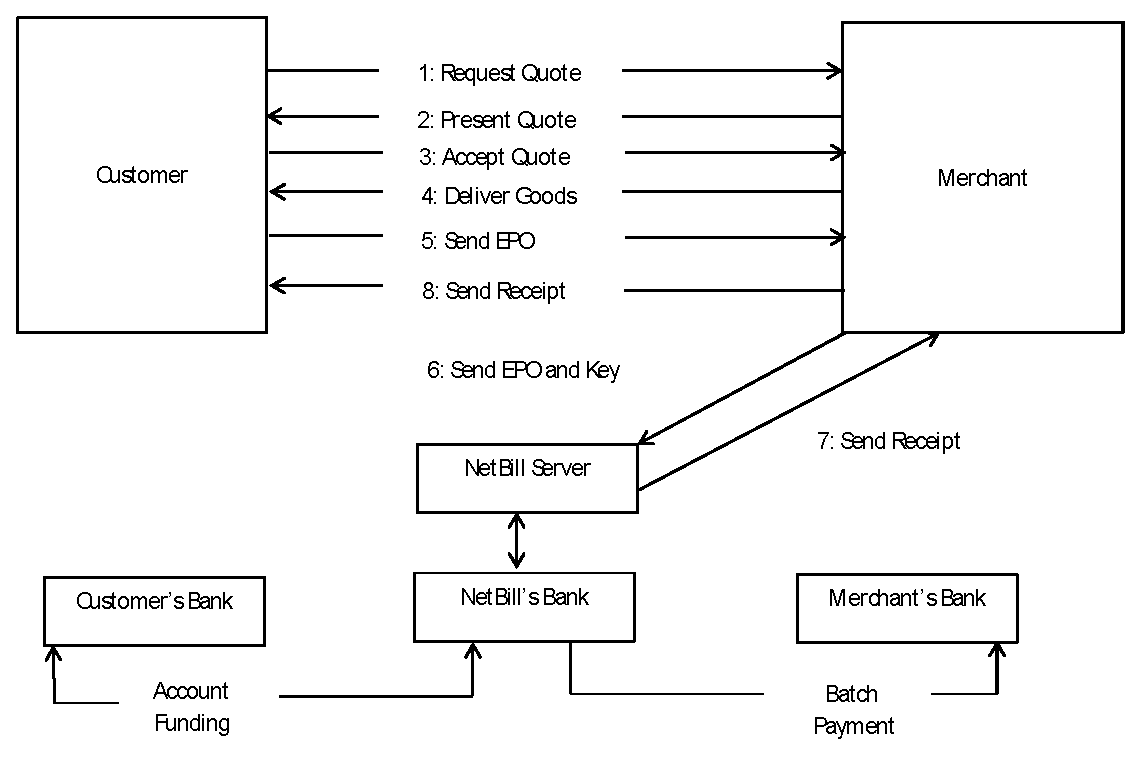
\includegraphics[width=12cm, height=8cm]{figures/figure1.eps}
        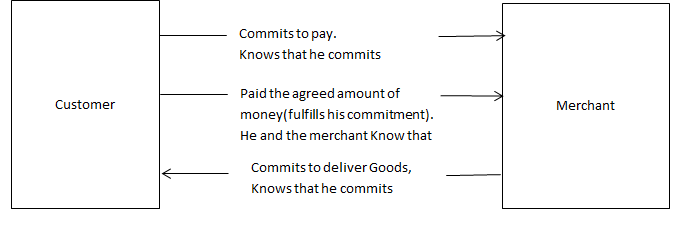
\includegraphics[width=1.0 \columnwidth]{figures/figure7.png}
        %%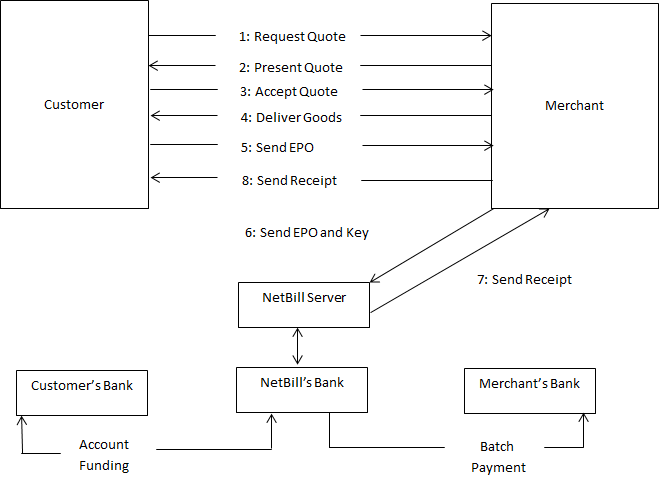
\includegraphics[scale=0.5]{figure1}
        %\caption{The NetBill payment protocol} \label{figure7}
    \end{figure}
    \end{frame}
%%%%%%%%%%%%%%%%%%%%%%%%%%%%%%%%%%%%%%%%%%%%%%%%%%%%%%%%%%%%%%%%%%%%%%%%%%%%%%
\begin{frame}{Problems and Research Questions}

\begin{itemize}
    \item \textbf{How can we model the
        community of agent-based services in order to maximize the utility
        of involved users, web services and community organizers?}.
        \begin{itemize}
            \item Most of the recent work on communities of
            services are either user-centric and focus on user satisfaction
            or system-centric and focus on the whole system throughput, performance and utilization.
        \end{itemize}


    \item \textbf{How can we model fair and stable communities as coalitions
        of agent-based web services?}.
        \begin{itemize}
            \item All parties involved are self-interest agents and have the authority to deviate leave the community if they can improve their income in some other ways.
        \end{itemize}

\end{itemize}

\end{frame}
%%%%%%%%%%%%%%%%%%%%%%%%%%%%%%%%%%%%%%%%%%%%%%%%%%%%%%%%%%%%%%%%%%%%%%%%%%%%%%

\begin{frame}{Continue: Problems and Research Questions}
 \begin{itemize}
   \item \textbf{How can we model and analyze the cooperation
        among the community members in realistic, applicable and practical
        settings?}
        \begin{itemize}
            \item Modeling the preference and valuation functions considering the worth of all subsets of players in realistic cooperative scenarios
            \item Solution concepts complexity issues
        \end{itemize}

\end{itemize}
\end{frame}
%%%%%%%%%%%%%%%%%%%%%%%%%%%%%%%%%%%%%%%%%%%%%%%%%%%%%%%%%%%%%%%%%%%%%%%%%%%%%%%
%    \begin{frame}{Multi-Agent Systems MASs}
%        \begin{itemize}
%            \itemsep=.35cm
%        	\item Multi-Agent System (MAS).
%            %\item Autonomous agents.
%        	\item Knowledge in MASs.
%            \item Social commitments in MASs.
%        \end{itemize}
%\end{frame}

%%%%%%%%%%%%%%%%%%%%%%%%%%%%%%%%%%%%%%%%%%%%%%%%%%%%%%%%%%%%%%%%%%%%%%%%%%%%%%
\section{Background}
\begin{frame}{Presentation Outline}
    \begin{itemize}
     	\itemsep=.5cm
    	\item Introduction
    	\item {\bf Background and Literature Review}
    	\item Proposed Research
        \item Contributions and Research Activities
    	\item Time Line
    \end{itemize}
\end{frame}

%%%%%%%%%%%%%%%%%%%%%%%%%%%%%%%% frame9 Background and Literature Review %%%%%%%%%%%%%%%%%%%%%%%%%%%%%%%%%%%%%
%%%%%%%%%%%%%%%%%%%%%%%%%%%%%%%%%%%%%%%%%%%%%%%%%%%%%%%%%%%%%%%%%%%%%%%%%%%%%%
\subsection{Communities of Web Services}
    \begin{frame}{Community of Web Services}
        Communities of Web Services
        \begin{itemize}
            \item Ease and improve the process of Web services discovery in an open environment like the Internet
        	\item Improve service quality, availability and responsiveness
        \end{itemize}

        \begin{figure}[htbp]
            \centering
            %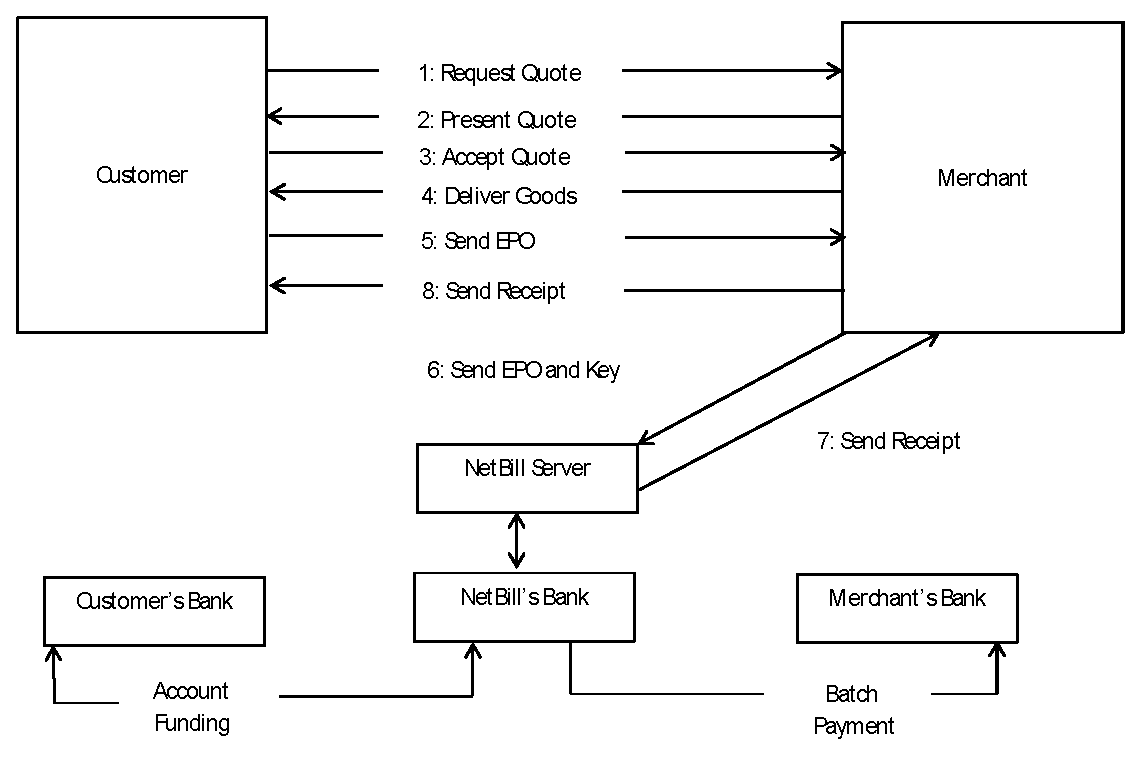
\includegraphics[width=12cm, height=8cm]{figures/figure1.eps}
            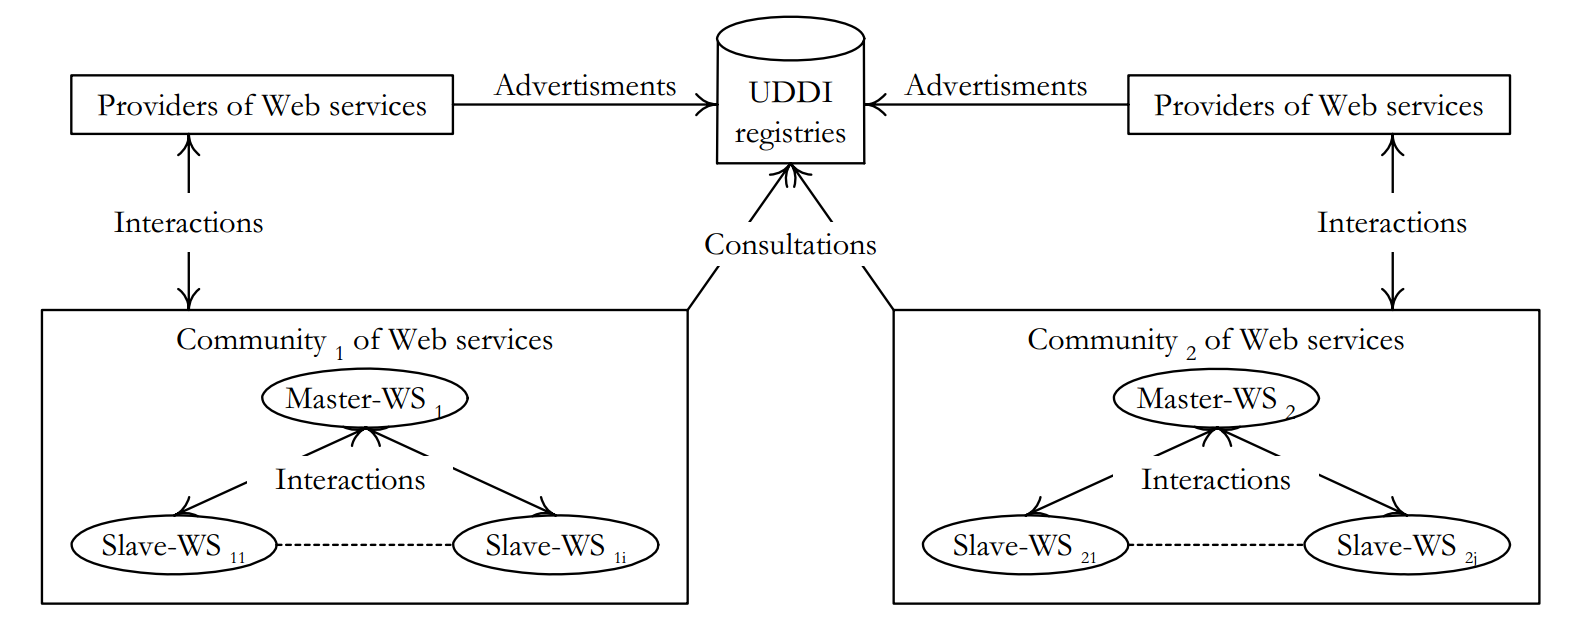
\includegraphics[width=1.0 \columnwidth]{figures/wscommunity2.png}
            %%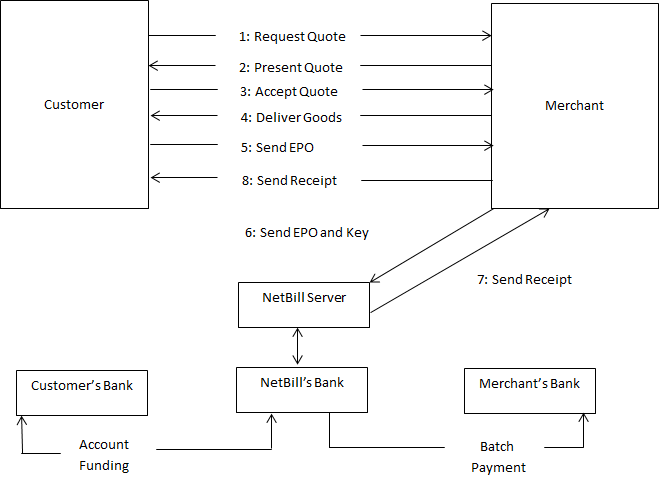
\includegraphics[scale=0.5]{figure1}
            %\caption{The NetBill payment protocol} \label{figure7}
        \end{figure}

    \end{frame}
%%%%%%%%%%%%%%%%%%%%%%%%%%%%%%%% frame10 Background and Literature Review %%%%%%%%%%%%%%%%%%%%%%%%%%%%%%%%%%%%%
%%%%%%%%%%%%%%%%%%%%%%%%%%%%%%%%%%%%%%%%%%%%%%%%%%%%%%%%%%%%%%%%%%%%%%%%%%%%%%
%\subsection{Social commitments in MASs}
    \begin{frame}{Communities of Web Services}
        Communities of Web Services
        \begin{itemize}
            \itemsep=.35cm
        	\item \textbf{Communities of web services operations}
            \begin{itemize}
              \item Community Development
              \item Web Services Attraction and Retention
              \item Web Service Selection
            \end{itemize}                      	      	
        \end{itemize}

        \begin{figure}[htbp]
            \centering
            %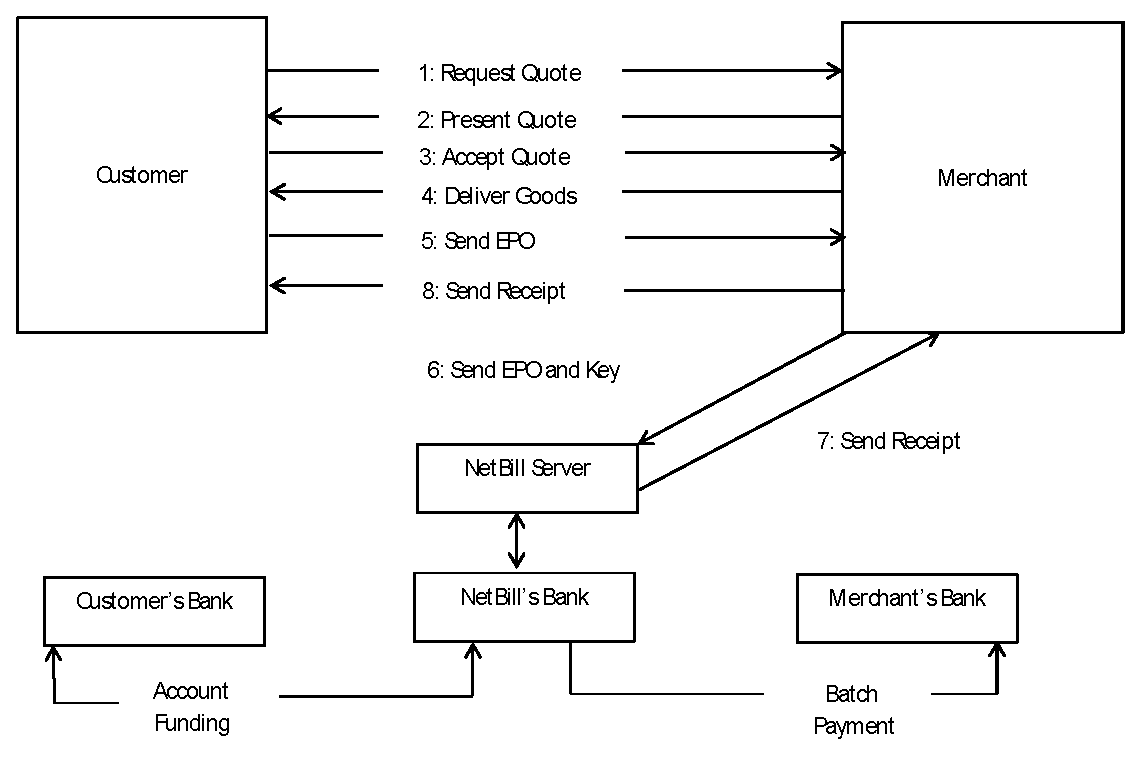
\includegraphics[width=12cm, height=8cm]{figures/figure1.eps}
            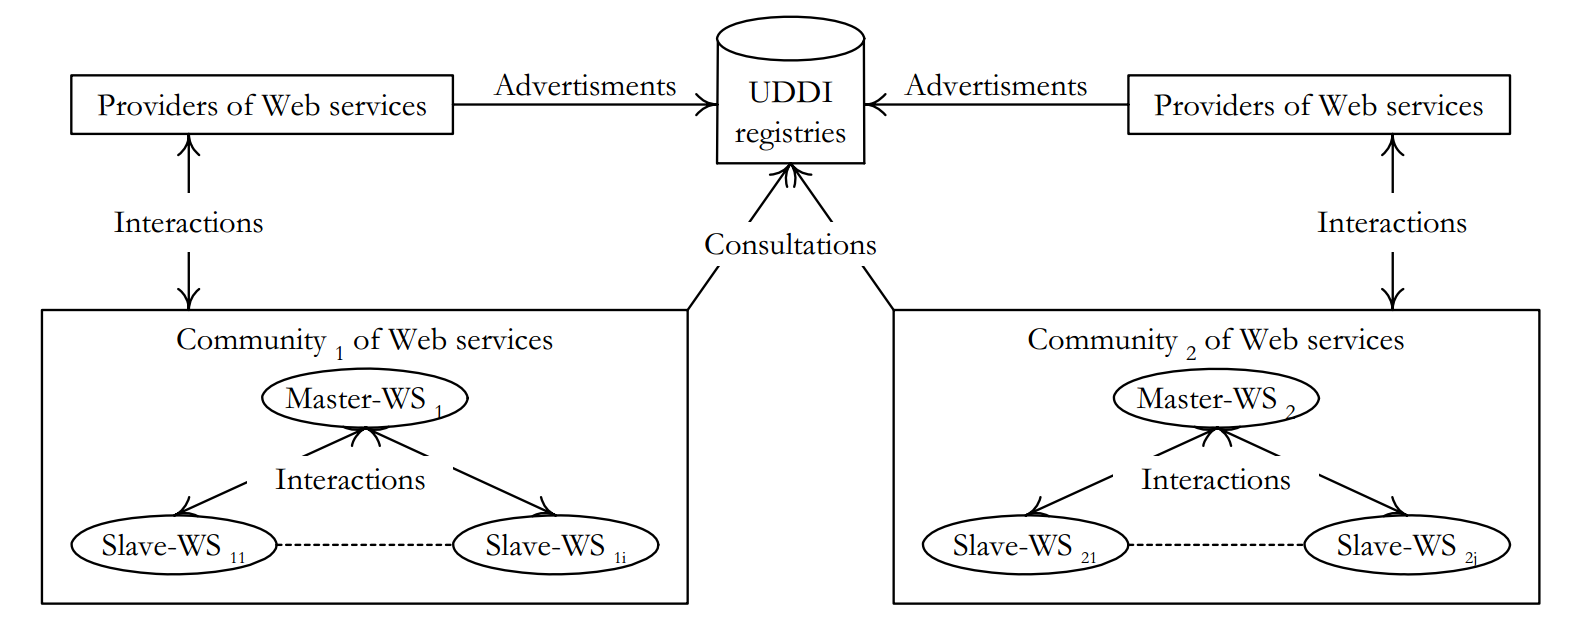
\includegraphics[width=1.0 \columnwidth]{figures/wscommunity2.png}
            %%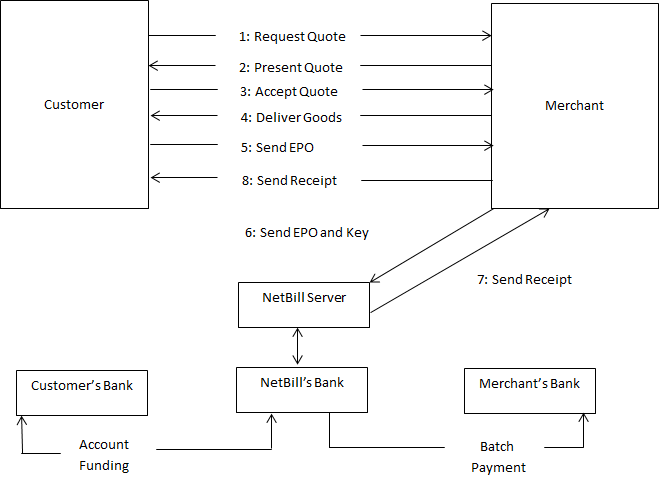
\includegraphics[scale=0.5]{figure1}
            %\caption{The NetBill payment protocol} \label{figure7}
        \end{figure}
    \end{frame}
%%%%%%%%%%%%%%%%%%%%%%%%%%%%%%%% frame11 Background and Literature Review %%%%%%%%%%%%%%%%%%%%%%%%%%%%%%%%%%%%%

%%%%%%%%%%%%%%%%%%%%%%%%%%%%%%%%%%%%%%%%%%%%%%%%%%%%%%%%%%%%%%%%%%%%%%%%%%%%%%
\subsection{Cooperative Game Theory}

    \begin{frame}{Cooperative Game Theory}
      \begin{itemize}
         \item Cooperative games are a branch of game theory that models cooperation or collaboration between agents.
         \begin{itemize}
            \item A set of tasks needs to be performed, they require different expertise.
            \item Agents do not have enough resource on their own to perform a task.
            \item Find complementary agents to perform the tasks.
            \begin{itemize}
                \item robots have the ability to move objects in a plant, but multiple robots are required to move a heavy box.
                \item transportation domain: agents are trucks, trains, airplanes, ships... a task is a good to be transported.
            \end{itemize}
        \end{itemize}
        \item \textbf{issues:}
            \begin{itemize}
                \item What coalition to form?
                \item How to reward each each member when a task is completed?
            \end{itemize}
      \end{itemize}
    \end{frame}

%%%%%%%%%%%%%%%%%%%%%%%%%%%%%%%% frame14 Background and Literature Review %%%%%%%%%%%%%%%%%%%%%%%%%%%%%%%%%%%%%
%%%%%%%%%%%%%%%%%%%%%%%%%%%%%%%%%%%%%%%%%%%%%%%%%%%%%%%%%%%%%%%%%%%%%%%%%%%%%%
\begin{frame}{The Classic Problem}
    We have a population $N$ of $n$ agents.
    \begin{definition} [Coalition]~\\
       A coalition $C$ is a set of agents: $C \in 2^N$.
        \begin{itemize}
            \item $N$ is the set of all agents (or players)
            \item $v:2^N \rightarrow R$ is the \emph{valuation function}. For $C \subseteq N$, $v(C)$ is the value obtained by the coalition $C$
        \end{itemize}
    \end{definition}

    \begin{itemize}
        \item \textbf{problem:} a game $(N,v)$, and we assume all agents in $N$ want to cooperate.
        \item \textbf{solution:} a payoff distribution $x \in R^n$ that provides a value to individual agents.

        \begin{itemize}
            \item What are the interesting properties that $x$ should satisfy?
            \item How to determine the payoff vector $x$?
        \end{itemize}

    \end{itemize}
\end{frame}
%%%%%%%%%%%%%%%%%%%%%%%%%%%%%%%%%%%%%%%%%%%%%%%%%%%%%%%%%%%%%%%%%%%%%%%%%%%%%%

\begin{frame}{An Example}

    \begin{center}
        $N = \{1,2,3\}$ \\
        $v(\{1\}) = 0, v(\{2\}) = 0, v(\{3\}) = 0$ \\
        $v(\{1,2\}) = 90$ \\
        $v(\{1,3\}) = 80$ \\
        $v(\{2,3\}) = 70$ \\
        $v(\{1,2,3\}) = 105$ \\
    \end{center}

    What should we do?
    \begin{itemize}
        \item form $\{1,2,3\}$ and share equally $(35,35,35)$?
        \item 3 can say to 1 ``let's form $\{1,3\}$ and share (40,0,40)''
        \item 2 can say to 1 ``let's form $\{1,2\}$ and share (45,45,0)''
        \item 3 can say to 2 ``OK, let's form $\{2,3\}$ and share (0,46,24)''
        \item 1 can say to 2 and 3, ``fine! $\{1,2,3\}$ and (33,47,25)''
        \item ...what is a good solution?
    \end{itemize}

\end{frame}

%%%%%%%%%%%%%%%%%%%%%%%%%%%%%%%% frame15 outline page

%%%%%%%%%%%%%%%%%%%%%%%%%%%%%%%%%%%%%%%%%%%%%%%%%%%%%%%%%%%%%%%%%%%%%%%%%%%%%%
\begin{frame}{Transferable and Non Transferable Utility Games}
    \begin{itemize}
        \item \textbf{Games with Transferable Utility (TU games)}
        \begin{itemize}
            \item Utility is worth the same for all agents
            \item Utility can be {\color{red} compared} or {\color{red} transfered} between agents.
            \item Irrespective of the division of the coalitional payoff, members of the coalition enjoy the same total utility.
        \end{itemize}


        \begin{definition} [Valuation or Characteristic function]\label{dfn:valuationfunction}
            A \emph{valuation function v} associates a real number $v(C)$ to any subset $C \subseteq N$, i.e., $v:2^N \rightarrow R$ \\
            A {\color{blue}\emph{TU game}} is a pair $(N,v)$ where $N$ is a set of agents and where $v$ is a valuation function.
        \end{definition}



        \item \textbf{Games with Non Transferable Utility (NTU games)} \\
            Agents have different preferences over coalitions and rewards. Non-monetary rewards, i.e. item allocation type of problems where items have different values for different players.
    \end{itemize}

\end{frame}
%%%%%%%%%%%%%%%%%%%%%%%%%%%%%%%%%%%%%%%%%%%%%%%%%%%%%%%%%%%%%%%%%%%%%%%%%%%%%%%
\begin{frame}{Some properties of valuation functions}
    $\forall C_1,C_2 \subseteq N | C_1 \bigcap C_2 = \emptyset, i \in N, i \notin C_1$
    \begin{itemize}
        \item {\color{red} additive:} $v(C_1 \bigcup C_2) = v(C_1) + v(C_2)$
        \item {\color{red} super additive:} $v(C_1 \bigcup C_2) \geq v(C_1) + v(C_2)$ This is satisfied is many applications, or bigger coalitions will not form.
        \item {\color{red} weekly super additive:} $v(C_1 \bigcup \{i\}) \geq v(C_1) + v(\{i\})$
        \item {\color{red} subadditive:} $v(C_1 \bigcup C_2) \leq v(C_1) + v(C_2)$
    \end{itemize}

    $\forall C_1,C_2 \subseteq N$
    \begin{itemize}
        \item {\color{red} convex:} $v(C_1) + v(C_2) \leq v(C_1 \bigcup C_2) + v(C_1 \bigcap C_2)$ Convexity has important properties in cooperative game theory solution concepts.
    \end{itemize}
\end{frame}
%%%%%%%%%%%%%%%%%%%%%%%%%%%%%%%%%%%%%%%%%%%%%%%%%%%%%%%%%%%%%%%%%%%%%%%%%%%%%%
\begin{frame}{Solution properties}
    Let $x \in R^n$ be a solution of the TU game $(N,v)$
    \begin{itemize}
        \item {\color{red} Feasible solution:} $\sum_{i \in N} x(i) \leq v(N)$
        \item {\color{red} Efficiency:} $x(N) = v(N)$
        \begin{itemize}
            \item the payoff distribution is an allocation of the entire worth of the grand coalition to all agents
        \end{itemize}
        \item {\color{red} Individual rationality:} $\forall i \in N, x(i) \geq v(\{i\})$
        \begin{itemize}
            \item player obtains at least its self-value of payoff
        \end{itemize}
        \item {\color{red} Group rationality:} $\forall C \subseteq N, \sum_{i \in N} x(i) \geq v(C)$
    \end{itemize}

    \vspace{0.2cm}

    An {\color{red} imputation} is a payoff distribution $x$ that is efficient and individual rational.

\end{frame}
%%%%%%%%%%%%%%%%%%%%%%%%%%%%%%%%%%%%%%%%%%%%%%%%%%%%%%%%%%%%%%%%%%%%%%%%%%
\begin{frame}{Stability}
    \begin{itemize}
        \item We all want to work together and get $v(N)$, but we all have different views about how to share the fruits of our work. We can use the values of other coalitions as arguments in favor of a distribution.
        \item A condition for a coalition to form:
            {\color{red}all} agents prefer to be in it. i.e., none of the participants wishes she were in a different coalition or by herself {\color{red} $\Rightarrow Stability$ }
        \item The {\color{red} core} is a stability concepts for which no agents prefer to deviate to form a different coalition.
        \item Is the coalition stable $\Leftrightarrow$ Is the core non-empty
    \end{itemize}
\end{frame}
%%%%%%%%%%%%%%%%%%%%%%%%%%%%%%%%%%%%%%%%%%%%%%%%%%%%%%%%%%%%%%%%%%%%%%%%%%%%%
\begin{frame}{Solution Concepts: Core}
    CTLC logic is an extension of CTL logic with modalities for reasoning about \textbf{commitments and their fulfillment}.
    \begin{definition} [Imputation]\label{dfn:imputationbig}
        An {\color{red}imputation} is a payoff distribution $x$ that is efficient and individually rational.
        \begin{itemize}
            \item $\sum_{i \in N} x(i) = v(N)$ (efficiency)
            \item for all $i \in N, x_i \geq v(\{i\})$ (individual rationality)
        \end{itemize}
    \end{definition}

    \begin{definition} [Group rationality]\label{dfn:grouprationality}
        $\forall C \subseteq N, \sum_{i \in N} x(i) \geq v(C)$
    \end{definition}
\end{frame}
%%%%%%%%%%%%%%%%%%%%%%%%%%%%%%%%%%%%%%%%%%%%%%%%%%%%%%%%%%%%%%%%%%%%%%%%%%%%%%
\begin{frame} {Solution Concepts: Core}
    The core relates to the stability of the grand coalition: \\ No group of agents has any incentive to change coalition.
    \begin{definition}[$Core$ of a game $(N,v)$]\label{dfn:core}
        Let $(N,v)$ be a cooperative game, and assume they form the coalition $N$. The core of $(N,v)$ is the set:
        \vspace{0.1cm}
        \begin{center}
            $Core(N,v) = \{x \in R^n | x$ is a group rational imputation$\}$
        \end{center}
        Equivalently,
        \vspace{0.1cm}
        \begin{center}
            $Core(N,v) = \{x \in R^n | x(N) \leq v(N) \wedge x(C) \geq v(C) \forall C \subseteq N\}$
        \end{center}
    \end{definition}

\end{frame}
%%%%%%%%%%%%%%%%%%%%%%%%%%%%%%%%%%%%%%%%%%%%%%%%%%%%%%%%%%%%%%%%%%%%%%%%%%%%%%
\begin{frame} {Example: Core}

    \begin{center}
      $N = \{1,2\}$ \\
      $v(\{1\}) = 5, v(\{2\}) = 5$ \\
      $v(\{1,2\}) = 20$ \\
    \end{center}

    $Core(N,n) = \{(x_1,x_2) \in R^2 | x_1 \geq 5, x_2 \geq 5, x_1 + x_2 = 20\}$

    \begin{figure}[htbp]
        \centering
        %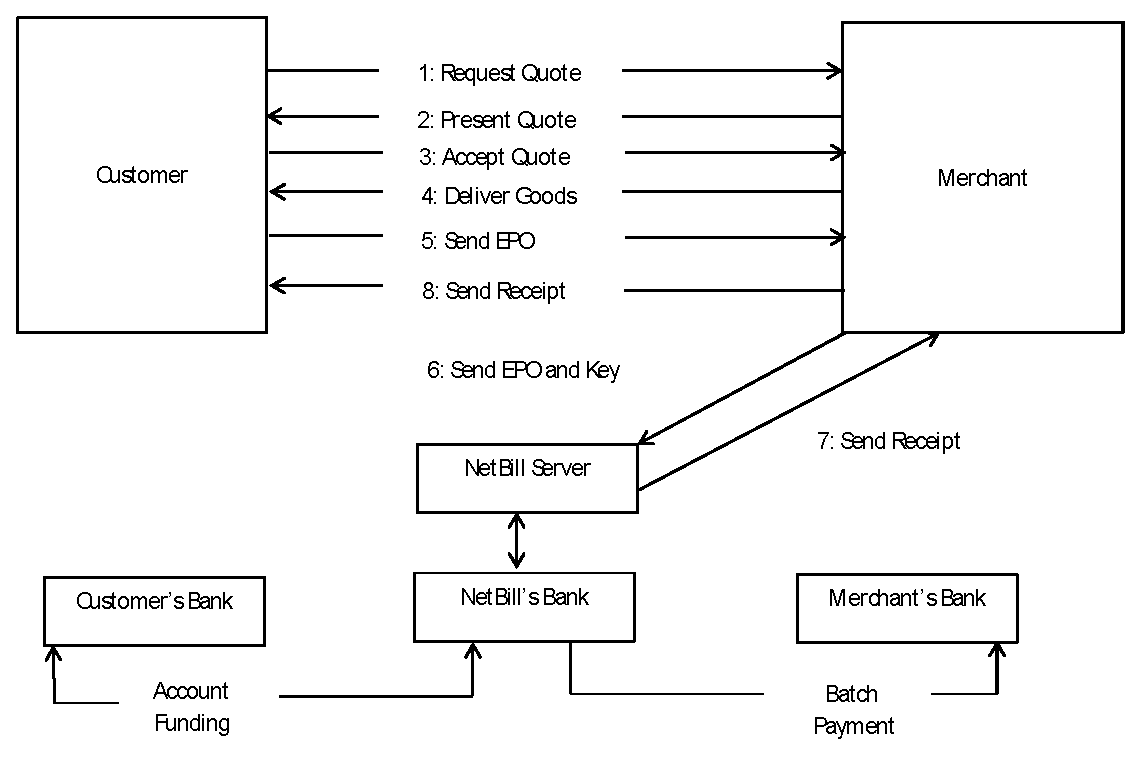
\includegraphics[width=12cm, height=8cm]{figures/figure1.eps}
        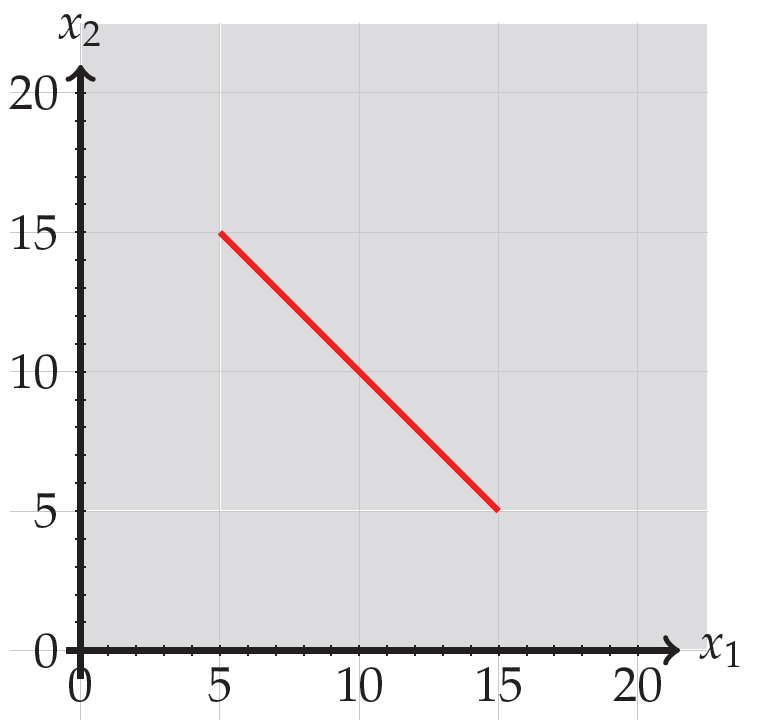
\includegraphics[width=0.3 \columnwidth]{figures/coreex1.png}
        %%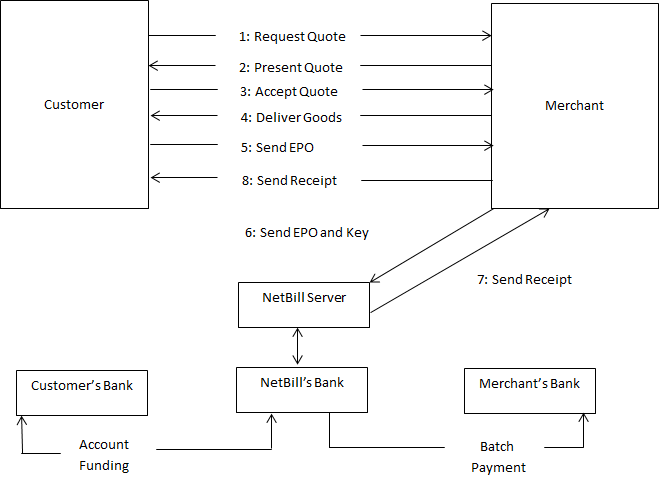
\includegraphics[scale=0.5]{figure1}
        %\caption{The NetBill payment protocol} \label{figure7}
    \end{figure}

    The core may not be fair: the core only considers stability.

\end{frame}
%%%%%%%%%%%%%%%%%%%%%%%%%%%%%%%%%%%%%%%%%%%%%%%%%%%%%%%%%%%%%%%%%%%%%%%%%%%%%
\begin{frame}{Solution Concepts: Shapley Value}
    \begin{definition} [Marginal contribution]\label{dfn:marginalcontribution}
        The {\color{red}marginal contribution} of agent $i$ for a coalition $C \subseteq N \backslash \{i\}$ is $mc_i(C) = v(C \cup \{i\}) - v(C)$
    \end{definition}

    \begin{itemize}
        \item By considering average marginal contribution over all possible subset of coalitions, we can achieve a fair distribution.\\
        \item Let $\prod(N)$ denote the set of all permutations of the sequence $(1,...n)$. Therefore: $\phi_i(N,v) = \frac{\sum_{\sigma \in \phi_i(N)}}{mc(\sigma)}$
    \end{itemize}

    \begin{definition} [Shapley Value]\label{dfn:shapleyvalue}
        Given a coalitional game $(N,v)$, the Shapley value of player $i$ is given by: \\
        $\phi_i(N,v) = \sum_{S \subseteq N \backslash \left\{i\right\} } \frac{|S|! (|N|-|S|-1)!}{|N|!} (v(S \cup \left\{i\right\}) - v(S))$
    \end{definition}
\end{frame}
%%%%%%%%%%%%%%%%%%%%%%%%%%%%%%%%%%%%%%%%%%%%%%%%%%%%%%%%%%%%%%%%%%%%%%%%%%%%%%%
\begin{frame}{Some properties}
    \begin{itemize}
        \item The core may not always be non-empty
        \item Shapley value always exists and is unique.
        \item When the valuation function is {\color{red}superadditive}, the Shapley value is {\color{red}individually rational}, i.e., it is an imputation.
        \item When the valuation function is {\color{red}convex}, the Shapley value is also group rational, hence, it is in the {\color{red}core}.
        \item A convex game has a non-empty core
        \item There are other well-known solution concepts: The bargaining set, The nucleolus and The nucleolus.
    \end{itemize}
\end{frame}
%%%%%%%%%%%%%%%%%%%%%%%%%%%%%%%%%%%%%%%%%%%%%%%%%%%%%%%%%%%%%%%%%%%%%%%%%%%%%%%
\begin{frame}{$\epsilon$-Core}
    \begin{itemize}
        \item The core may not always be non-empty
        \item (To add some items)
    \end{itemize}
\end{frame}
%%%%%%%%%%%%%%%%%%%%%%%%%%%%%%%%%%%%%%%%%%%%%%%%%%%%%%%%%%%%%%%%%%%%%%%%%%%%%%%
\begin{frame}{Coalition Structures}
    \begin{itemize}
        \item To reach a stable partition having many coalitions.
        \item (To add some items)
    \end{itemize}
\end{frame}

%%%%%%%%%%%%%%%%%%%%%%%%%%%%%%%%%%%%%%%%%%%%%%%%%%%%%%%%%%%%%%%%%%%%%%%%%%%%%%
%%%%%%%%%%%%%%%%%%%%%%%%%%%%%%%%%%%%%%%%%%%%%%%%%%%%%%%%%%%%%%%%%%%%%%%%%%%%%%%
\section{Proposed Research}
\begin{frame}{Presentation Outline}
    \begin{itemize}
     	\itemsep=.5cm
    	\item Introduction
    	\item Background and Literature Review
    	\item {\bf Proposed Research}
        \item Contribution and Research Activities
    	\item Time Line
    \end{itemize}
\end{frame}

%%%%%%%%%%%%%%%%%%%%%%%%%%%%%%%% frame16 Proposed Research %%%%%%%%%%%%%%%%%%%%%%%%%%%%%%%%%%%%%
%%%%%%%%%%%%%%%%%%%%%%%%%%%%%%%%%%%%%%%%%%%%%%%%%%%%%%%%%%%%%%%%%%%%%%%%%%%%%%%
\subsection{Problem Formulation and Modeling}

\begin{frame}{Problem Formulation and Modeling}
    \begin{itemize}
        \item Communities are robust service providers with well established market share and reputation
        \item The community is characterized by a request rate $R_C$
        \item Web services can perform tasks with some throughput rate ($Th_{ws}$)
        \item Web services come with different values of $QoS_{ws}$ for different metrics.
        \item 123
    \end{itemize}
\end{frame}

%%%%%%%%%%%%%%%%%%%%%%%%%%%%%%%%%%%%%%%%%%%%%%%%%%%%%%%%%%%%%%%%%%%%%%%%%%%%%%%
\begin{frame}{Task distribution}
    \begin{itemize}
        \item Our model uses a slightly modified $weighted fair queuing$ method for task distribution rather than Contract-Net.
        \item All the input flow is multiplexed amount different web services with weights proportional to their throughput value ($Th_{ws}$).
        \item Queues will happen if $R_C$ is more than summation web services throughput.
        \item Weighted task rate of: $R_C \times \frac{Th_{ws}}{\sum_{ws}{Th_{ws}}}$ or $Th_{ws}$
    \end{itemize}
    \begin{figure}[htbp]
        \centering
        %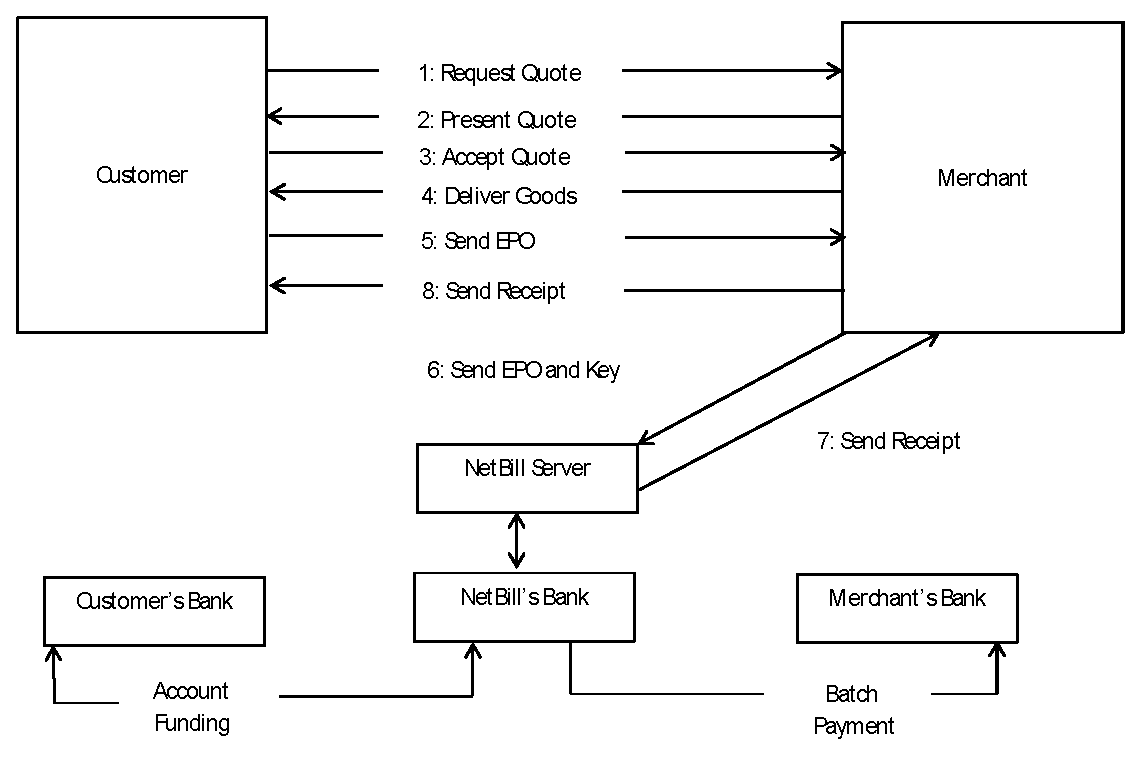
\includegraphics[width=12cm, height=8cm]{figures/figure1.eps}
        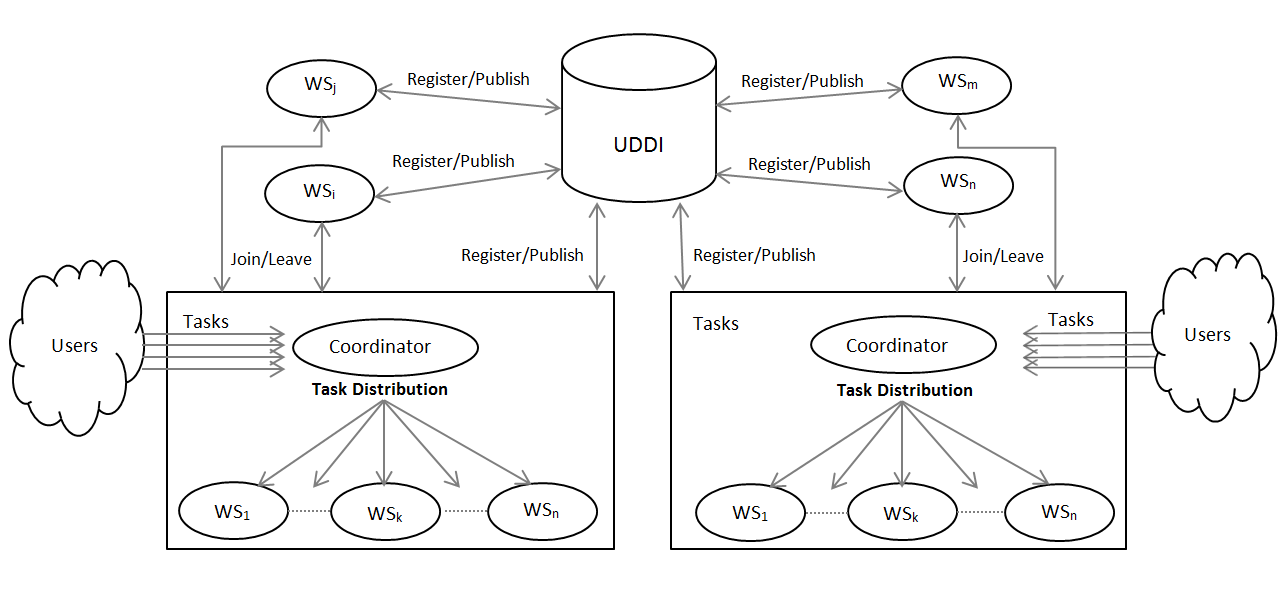
\includegraphics[width=0.8 \columnwidth]{figures/community.png}
        %%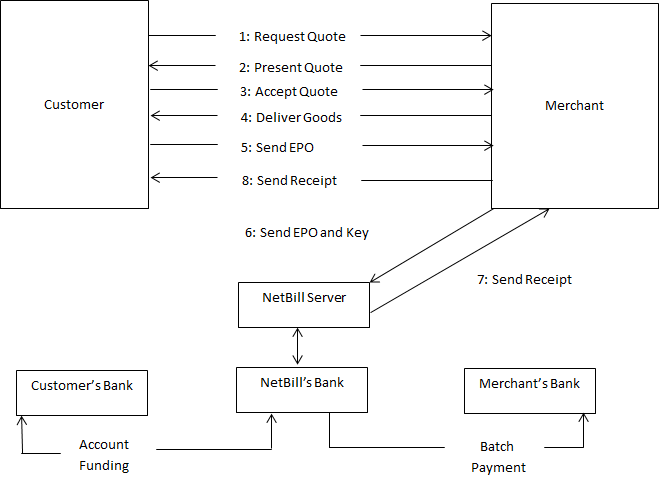
\includegraphics[scale=0.5]{figure1}
        %\caption{The NetBill payment protocol} \label{figure7}
    \end{figure}
\end{frame}

%%%%%%%%%%%%%%%%%%%%%%%%%%%%%%%%%%%%%%%%%%%%%%%%%%%%%%%%%%%%%%%%%%%%%%%%%%%%%%%
\begin{frame}{Community Revenue}
    \begin{itemize}
        \item Maximum potential output of a community:
            \begin{equation*}
                PO(C) = \sum_{ws \in C}{(T_{ws} \times QoS_{ws})}
            \end{equation*}
        \item if $Th_{ws} > R_C$, the community cannot perform at its maximum potential.
        \item Actual output:
            \begin{equation}\label{out_c}
                Out(C) = \left\{
                  \begin{array}{l l}
                    PO(C) & \quad \text{if $\sum_{ws}{Th_{ws}} \leq R_{C}$}\\
                    PO(C) \times \frac{R_{C}}{\sum_{ws}{Th_{ws}}} & \quad \text{if $\sum_{ws}{Th_{ws}} > R_{C}$}
                  \end{array} \right.
            \end{equation}
    \end{itemize}
\end{frame}

%%%%%%%%%%%%%%%%%%%%%%%%%%%%%%%%%%%%%%%%%%%%%%%%%%%%%%%%%%%%%%%%%%%%%%%%%%%%%%%
\begin{frame}{Example 1}
    \begin{table}[!t]
    \renewcommand{\arraystretch}{1.3}
    % if using array.sty, it might be a good idea to tweak the value of
    % \extrarowheight as needed to properly center the text within the cells
    \label{example_1}
    \centering
    \begin{tabular}{c c c c}
    \hline
    $WS$ & $QoS_{ws}$ & $Th_{ws}$ & $Th_{ws} \times QoS_{ws}$\\
    \hline
    1 & 0.8 & 4 & 3.2\\
    2 & 0.8 & 5 & 4.0\\
    3 & 0.8 & 3 & 2.4\\
    \hline
    \end{tabular}
    \end{table}

    \begin{table}[!t]
    \renewcommand{\arraystretch}{1.3}
    % if using array.sty, it might be a good idea to tweak the value of
    % \extrarowheight as needed to properly center the text within the cells
    % \caption{Three web services}
    \label{example_1_2}
    \centering
    \begin{tabular}{c c || c c}
    \hline
    Community & Worth & Community & Worth\\
    \hline
    $\left\{1\right\}$ & 3.2 & $\left\{1,2\right\}$ & 7.2\\
    $\left\{2\right\}$ & 4.0 & $\left\{1,3\right\}$ & 5.6\\
    $\left\{3\right\}$ & 2.4 & $\left\{2,3\right\}$ & 6.4\\
    $\left\{1,2,3\right\}$ & 8.0\\
    \hline
    Community $R_C$: 10\\
    \hline
    \end{tabular}
    \end{table}
\end{frame}

%%%%%%%%%%%%%%%%%%%%%%%%%%%%%%%%%%%%%%%%%%%%%%%%%%%%%%%%%%%%%%%%%%%%%%%%%%%%%%%
\begin{frame}{Example 2}
    \begin{table}[!t]
    \renewcommand{\arraystretch}{1.3}
    % if using array.sty, it might be a good idea to tweak the value of
    % \extrarowheight as needed to properly center the text within the cells
    \label{example_2}
    \centering
    \begin{tabular}{c c c c}
    \hline
    $WS$ & $QoS_{ws}$ & $Th_{ws}$ & $Th_{ws} \times QoS_{ws}$\\
    \hline
    1 & 0.8 & 5 & 4.0\\
    2 & 0.7 & 6 & 4.2\\
    3 & 0.7 & 4 & 2.8\\
    \hline
    \end{tabular}
    \end{table}

    \begin{table}[!t]
    \renewcommand{\arraystretch}{1.3}
    % if using array.sty, it might be a good idea to tweak the value of
    % \extrarowheight as needed to properly center the text within the cells
    % \caption{Three web services}
    \label{example_2_2}
    \centering
    \begin{tabular}{c c || c c}
    \hline
    Community & Worth & Community & Worth\\
    \hline
    $\left\{1\right\}$ & 4.0 & $\left\{1,2\right\}$ & 7.4\\
    $\left\{2\right\}$ & 4.2 & $\left\{1,3\right\}$ & 6.8\\
    $\left\{3\right\}$ & 2.8 & $\left\{2,3\right\}$ & 7.0\\
    $\left\{1,2,3\right\}$ & 7.3\\
    \hline
    Community $R_C$: 10\\
    \hline
    \end{tabular}
    \end{table}
\end{frame}

%%%%%%%%%%%%%%%%%%%%%%%%%%%%%%%%%%%%%%%%%%%%%%%%%%%%%%%%%%%%%%%%%%%%%%%%%%%%%%%
\begin{frame}{Example 3}
    \begin{table}[!t]
    \renewcommand{\arraystretch}{0.8}
    % if using array.sty, it might be a good idea to tweak the value of
    % \extrarowheight as needed to properly center the text within the cells
    \label{example_3}
    \centering
    \begin{tabular}{c c c c}
    \hline
    $WS$ & $QoS_{ws}$ & $Th_{ws}$ & $\text{\emph{Input Task Rate}}$\\
    \hline
    1 & 0.8 & 10 & 5\\
    2 & 0.8 & 20 & 5\\
    3 & 0.8 & 30 & 5\\
    \hline
    \end{tabular}
    \end{table}

    \begin{table}[!t]
    \renewcommand{\arraystretch}{0.8}
    % if using array.sty, it might be a good idea to tweak the value of
    % \extrarowheight as needed to properly center the text within the cells
    % \caption{Three web services}
    \label{example_3_2}
    \centering
    \begin{tabular}{c c || c c}
    \hline
    Community & Worth & Community & Worth\\
    \hline
    $\left\{C_{ms_1}\right\}$ & 0 & $\left\{C_{ms_2}\right\}$ & 0\\
    $\left\{C_{ms_1}, ws_1\right\}$ & 8 & $\left\{C_{ms_2}, ws_1\right\}$ & 8\\
    $\left\{C_{ms_1}, ws_2\right\}$ & 16 & $\left\{C_{ms_2}, ws_2\right\}$ & 16\\
    $\left\{C_{ms_1}, ws_3\right\}$ & 16 & $\left\{C_{ms_2}, ws_3\right\}$ & 24\\
    $\left\{C_{ms_1}, ws_1, ws_2\right\}$ & 16 & $\left\{C_{ms_2}, ws_1, ws_2\right\}$ & 24\\
    $\left\{C_{ms_1}, ws_1, ws_3\right\}$ & 16 & $\left\{C_{ms_2}, ws_1, ws_3\right\}$ & 32\\
    $\left\{C_{ms_1}, ws_2, ws_3\right\}$ & 16 & $\left\{C_{ms_2}, ws_2, ws_3\right\}$ & 32\\
    $\left\{C_{ms_1}, ws_1, ws_2, ws_3\right\}$ & 16 & $\left\{C_{ms_2}, ws_1, ws_2, ws_3\right\}$ & 32\\
    $\left\{C_{ms_1}, C_{ms_2}, ...\right\}$ & 0 & $\left\{ws_1\right\}$ & 6.8\\
    $\left\{ws_2\right\}$ & 4.2 & $\left\{ws_3\right\}$ & 6.8\\
    \hline
    Community $R_{C_1}$: 20 \\ Community $R_{C_2}$: 40\\
    \hline
    \end{tabular}
    \end{table}
\end{frame}

%%%%%%%%%%%%%%%%%%%%%%%%%%%%%%%% frame19 Proposed Research
%%%%%%%%%%%%%%%%%%%%%%%%%%%%%%%%%%%%%%%%%%%%%%%%%%%%%%%%%%%%%%%%%%%%%%%%%%%%%%%
\subsection{Web Service Cooperative Games}

%%%%%%%%%%%%%%%%%%%%%%%%%%%%%%%%%%%%%%%%%%%%%%%%%%%%%%%%%%%%%%%%%%%%%%%%%%%%%%%
\begin{frame}{Scenario One: Web Services and One Community}
    \begin{figure}[htbp]
        \centering
        %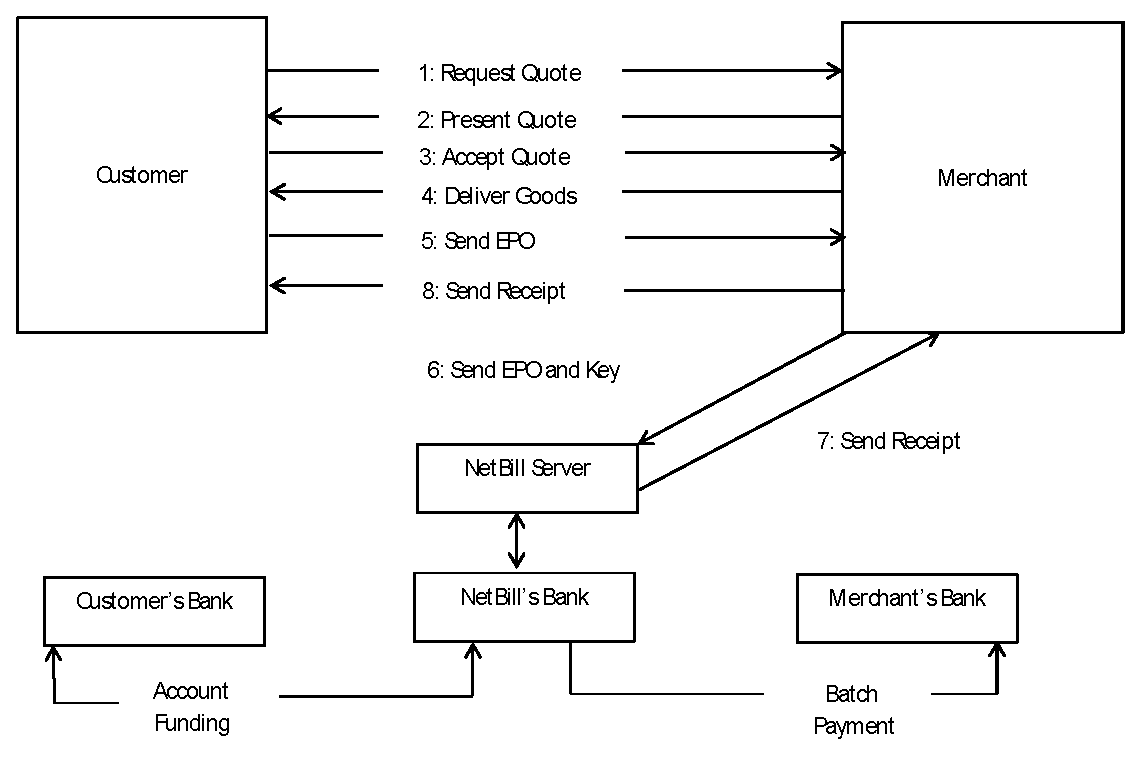
\includegraphics[width=12cm, height=8cm]{figures/figure1.eps}
        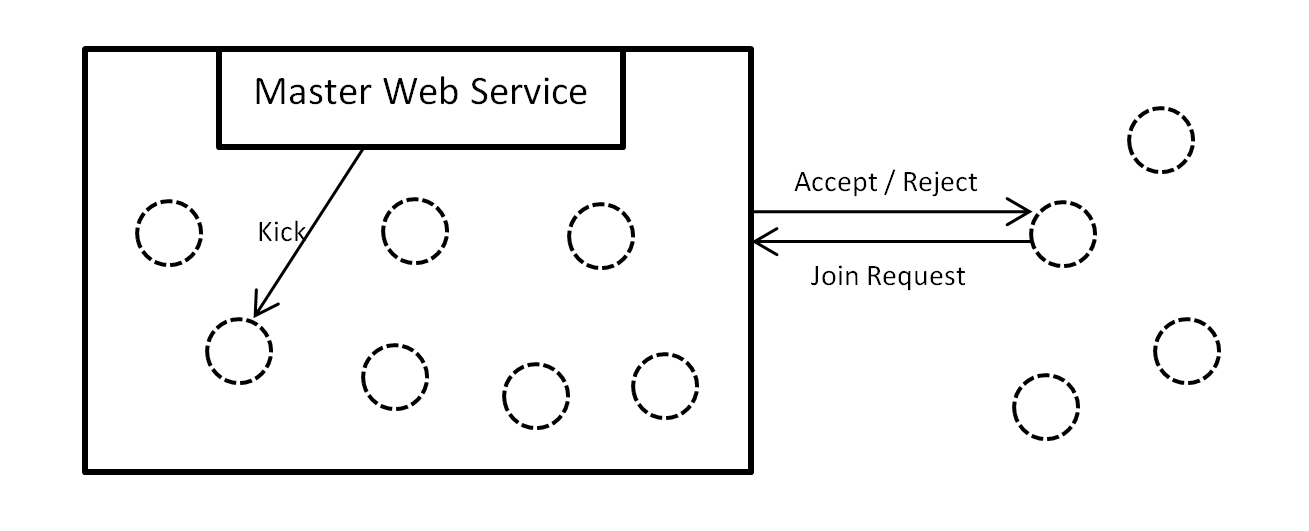
\includegraphics[width=0.8 \columnwidth]{figures/scenario1.png}
        %%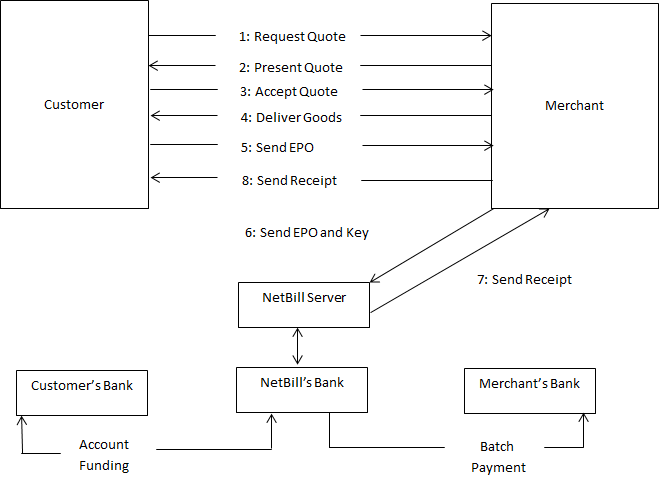
\includegraphics[scale=0.5]{figure1}
        %\caption{The NetBill payment protocol} \label{figure7}
    \end{figure}

    \begin{itemize}
        \item A typical WS community, where web services can join or leave
        \item $v(C) = Out(C)$
        \item Membership decision in made based on throughput and QoS of the web services.
        \item Community master needs to get quality web services to keep community stable, so other web services have no incentive to leave.
    \end{itemize}
       	
\end{frame}
%%%%%%%%%%%%%%%%%%%%%%%%%%%%%%%%%%%%%%%%%%%%%%%%%%%%%%%%%%%%%%%%%%%%%%%%%%%%%%%
\begin{frame}{Scenario One: Web Services and One Community}


    \begin{itemize}
        \item Upon receiving membership request the master web service checks if the coalition will be stable having the new member.
        \item If the game is convex, core exists.
        \item If the game is convex, shapley value is in core.
        \item Convexity Condition: 
        \item Community master needs to get quality web services to keep community stable, so other web services have no incentive to leave.
    \end{itemize}
       	
\end{frame}
%%%%%%%%%%%%%%%%%%%%%%%%%%%%%%%%%%%%%%%%%%%%%%%%%%%%%%%%%%%%%%%%%%%%%%%%%%%%%%%

\begin{frame}{Scenario One: Web Services and One Community}
    \begin{itemize}
        \item 123123
        \item 123123
        \item 123123
    \end{itemize}
    \begin{figure}[htbp]
        \centering
        %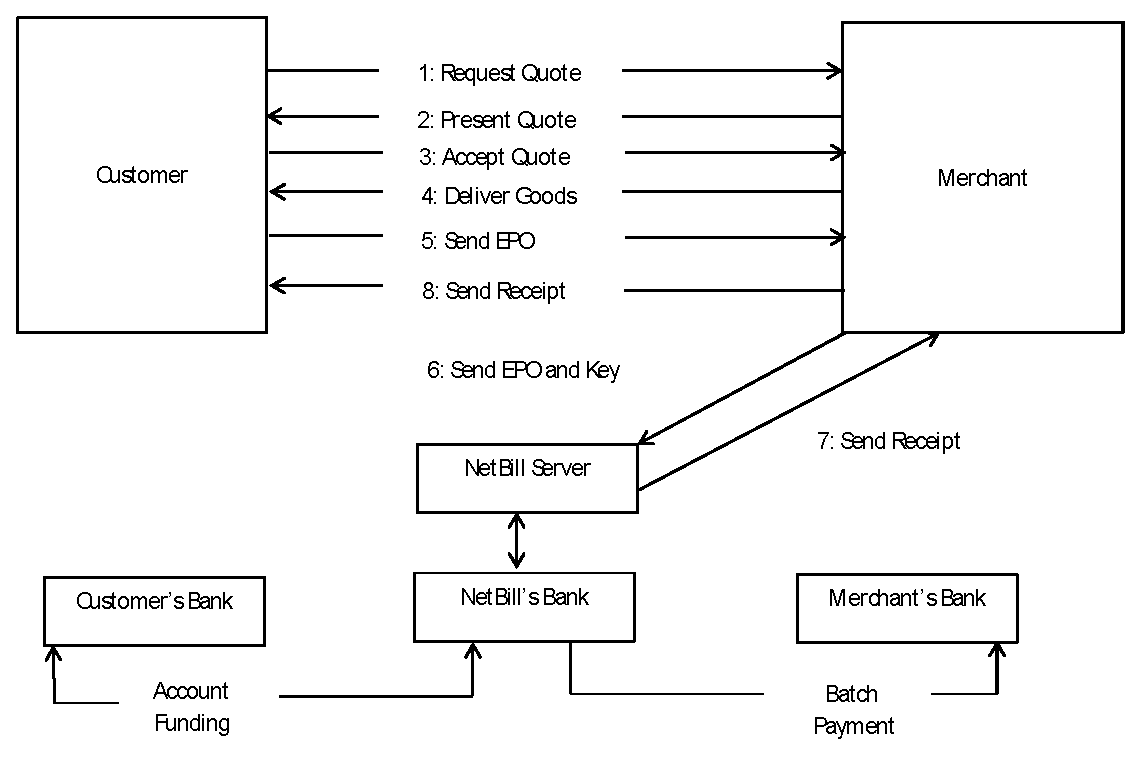
\includegraphics[width=12cm, height=8cm]{figures/figure1.eps}
        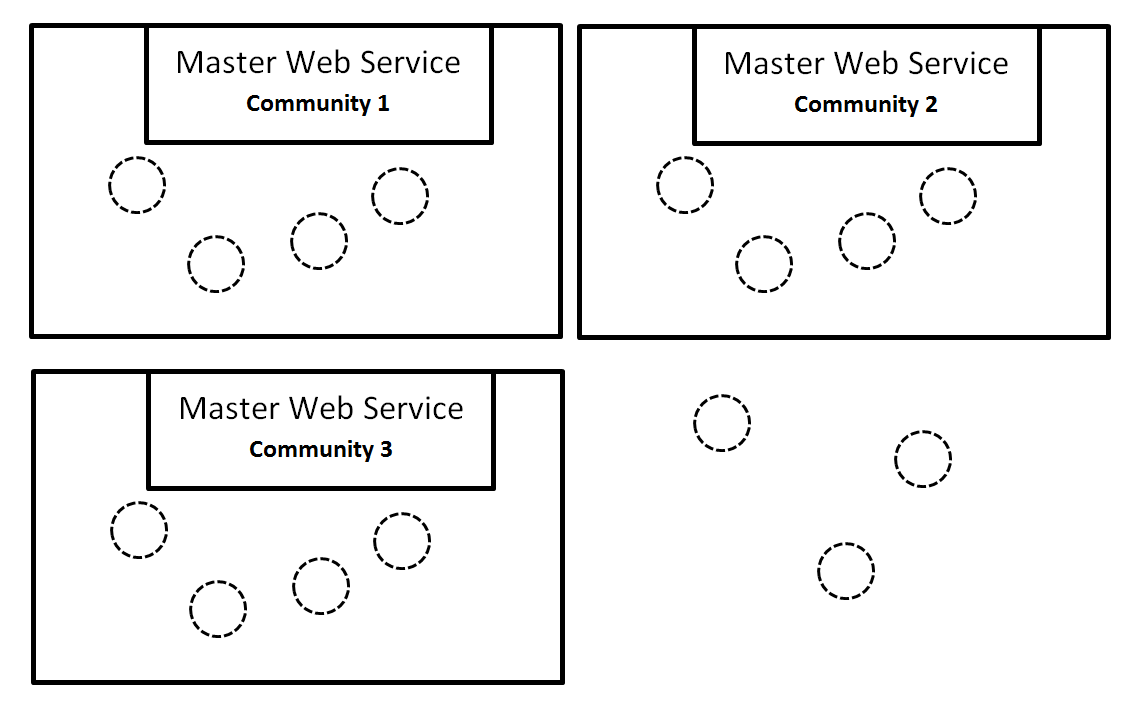
\includegraphics[width=0.8 \columnwidth]{figures/scenario2.png}
        %%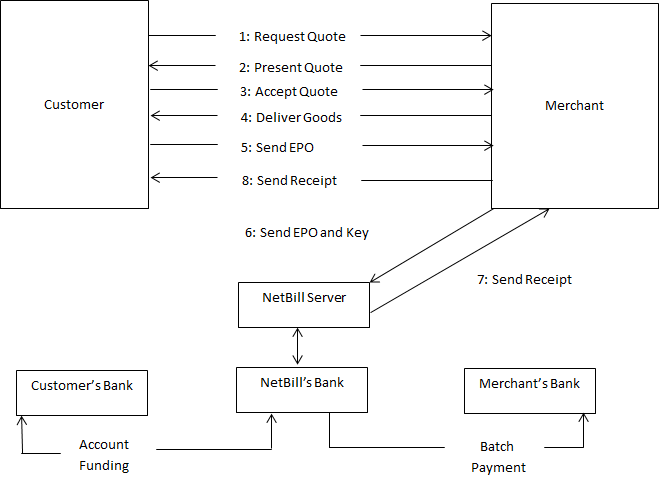
\includegraphics[scale=0.5]{figure1}
        %\caption{The NetBill payment protocol} \label{figure7}
    \end{figure}
       	
\end{frame}
%%%%%%%%%%%%%%%%%%%%%%%%%%%%%%%%%%%%%%%%%%%%%%%%%%%%%%%%%%%%%%%%%%%%%%%%%%%%%%%

\begin{frame}{Continue: Desiderata of Paradoxes}
 \begin{enumerate}
\vspace{0.2cm} \item [P3.][\textbf{Committing everything known
from others}]
$ K_i K_j \varphi \Rightarrow C_{j \rightarrow i} \varphi$ such that $ i \neq j$.

\textbf{Meaning:} An agent (the debtor) commits toward another
agent (the creditor) to bring about what the creditor knows about
the debtor's knowledge.\\
\textbf{Example 3:}\\
$K_{Cus} K_{Mer}$ $deliverGoods \Rightarrow$ $C_{Mer \rightarrow Cus}$
$deliverGoods$.

\vspace{0.2cm} \item [P4.][\textbf{Knowing about his own
commitment}]

$C_{i\rightarrow j} \varphi \Rightarrow K_i (C_{i\rightarrow j}
\varphi) $ where $i \neq j$.

\textbf{Meaning:} An agent knows about his commitment.


\textbf{Example 4:}\\
$C_{Cus \rightarrow Mer}$ $sendPayment $ $\Rightarrow K_{Cus}$ $(C_{Cus \rightarrow Mer}$ $sendPayment)$.
\end{enumerate}

        	
\end{frame}
%%%%%%%%%%%%%%%%%%%%%%%%%%%%%%%%%%%%%%%%%%%%%%%%%%%%%%%%%%%%%%%%%%%%%%%%%%%%%%%

%%%%%%%%%%%%%%%%%%%%%%%%%%%%%%%%%%%%%%%%%%%%%%%%%%%%%%%%%%%%%%%%%%%%%%%%%%%%%%%

\begin{frame}{Continue: Desiderata of Paradoxes}

\begin{figure}[htbp]
    \begin{center}
%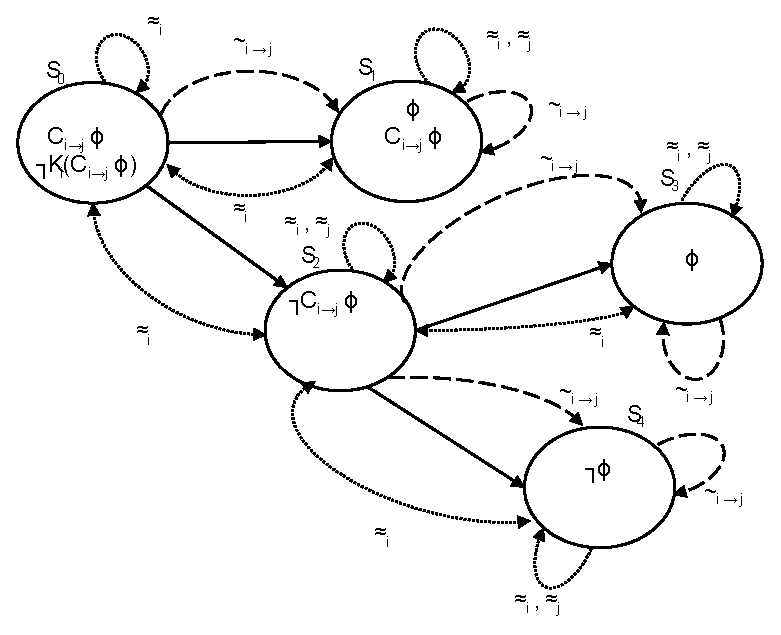
\includegraphics[width=10cm, height=5cm]{figures/figure2.eps}
    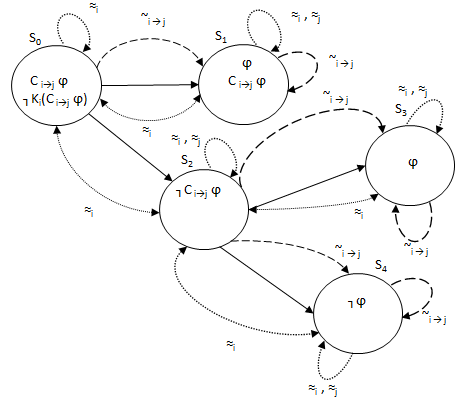
\includegraphics[width=.75 \columnwidth]{figures/figure2.png}
   % \caption{Model 1} \label{figure2}
    \end{center}
    \end{figure}
\end{frame}
%%%%%%%%%%%%%%%%%%%%%%%%%%%%%%%%%%%%%%%%%%%%%%%%%%%%%%%%%%%%%%%%%%%%%%%%%%%%%%%

\begin{frame}{Continue: Desiderata of Paradoxes}
\begin{enumerate}
\vspace{0.2cm} \item [P5.][\textbf{Knowing the content of his own
fulfilled commitment}]

$Fu (C _{i\rightarrow j} \varphi) \Rightarrow K _i \varphi$ where
$i \neq j$.

\textbf{Meaning:} An agent knows the content of his fulfilled
commitment.\\
\textbf{Example 5:}\\
$Fu (C _{Cus\rightarrow Mer} sendPayment) \Rightarrow K_{Cus}$ $sendPayment$.
\begin{figure}[htbp]
    \begin{center}
%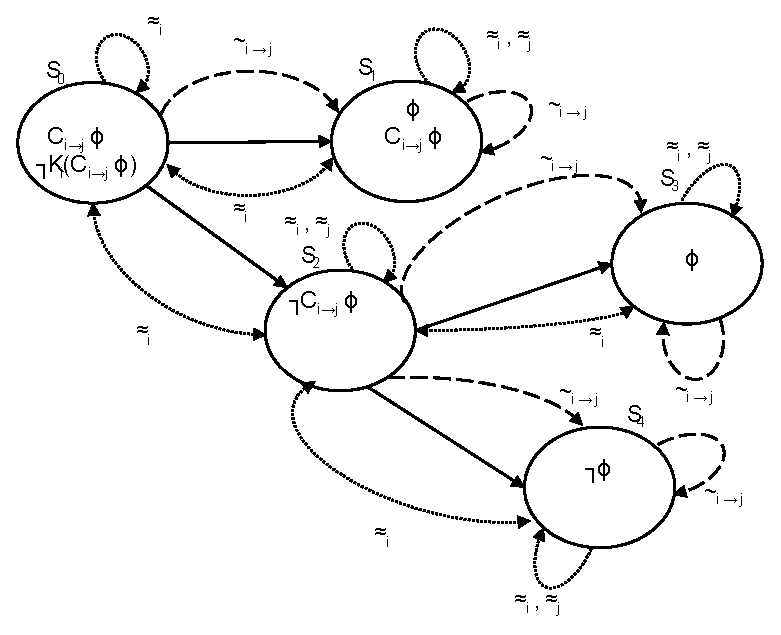
\includegraphics[width=10cm, height=5cm]{figures/figure2.eps}
    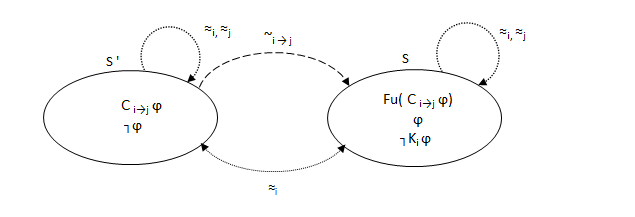
\includegraphics[width=.75 \columnwidth]{figures/figure3.png}
   % \caption{Model 2} \label{figure3}
    \end{center}
    \end{figure}

\end{enumerate}     	
\end{frame}
%%%%%%%%%%%%%%%%%%%%%%%%%%%%%%%% frame23 Proposed Research %%%%%%%%%%%%%%%%%%%%%%%%%%%%%%%%%%%%%
%%%%%%%%%%%%%%%%%%%%%%%%%%%%%%%%%%%%%%%%%%%%%%%%%%%%%%%%%%%%%%%%%%%%%%%%%%%%%%%

 \begin{frame}{Continue: Desiderata of Paradoxes}
 \begin{enumerate}

\vspace{0.2cm} \item [P6.][\textbf{Knowing the content of the
other's fulfilled commitment}]

$Fu (C _{i\rightarrow j} \varphi) \Rightarrow K_j \varphi$ where
$i \neq j$.

\textbf{Meaning:} The creditor knows the content of the debtor's
fulfilled commitment.\\
\textbf{Example 6:}\\
$ Fu (C_{cust \rightarrow Mer}$ $sendPayment)$ $\Rightarrow $ $k_{Mer} sendPayment$.
	\begin{figure}[htbp]
\begin{center}
%\includegraphics[width=12cm, height=5cm]{figures/figure4.eps}
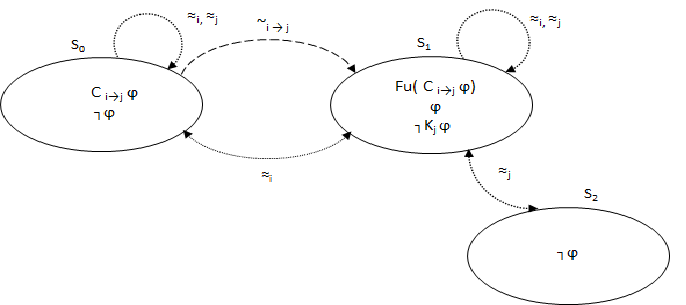
\includegraphics[width=.70 \columnwidth]{figures/figure4.png}
%\caption{Model 3} \label{figure4}
\end{center}
\end{figure}
\end{enumerate}
\end{frame}

%%%%%%%%%%%%%%%%%%%%%%%%%%%%%%%% frame24 Proposed Research %%%%%%%%%%%%%%%%%%%%%%%%%%%%%%%%%%%%%
%%%%%%%%%%%%%%%%%%%%%%%%%%%%%%%%%%%%%%%%%%%%%%%%%%%%%%%%%%%%%%%%%%%%%%%%%%%%%%
\begin{frame}{Continue: Desiderata of Paradoxes}
\begin{enumerate}
    \vspace{0.2cm} \item [P7.][\textbf{Knowing the commitment of the
other}]

$C_{i\rightarrow j} \varphi \Rightarrow AF K_j (C_{i\rightarrow j}
\varphi) $ where $i \neq j$.

\textbf{Meaning:} An agent should be aware of any commitments
directed towards him.\\
\textbf{Example 7:}\\
$C_{Mer \rightarrow Cus}$ $deliverGoods$ $\Rightarrow $ $AF K_{Cus}(C_{Mer \rightarrow Cus}$
$deliverGoods$).
\begin{figure}[htbp]
\centering
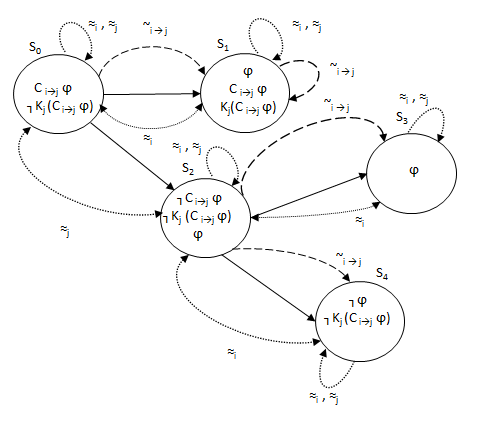
\includegraphics[width=.50 \columnwidth]{figures/figure5.png}
%\includegraphics[width=12cm, height=7cm]{figures/figure5.eps}
%\includegraphics[scale=0.5]{figure4.eps}
%\caption{Model 4} \label{figure5}
\end{figure}

\end{enumerate}
\end{frame}
%%%%%%%%%%%%%%%%%%%%%%%%%%%%%%%%%%%%%%%%%%%%%%%%%%%%%%%%%%%%%%%%%%%%%%%%%%%%%%%
\begin{frame}{Continue: Desiderata of Paradoxes}
\begin{enumerate}
    \vspace{0.2cm} \item [P8.][\textbf{Knowing the fulfillment of his
own commitment}]

$Fu(C _{i\rightarrow j} \varphi) \Rightarrow K_i Fu(C
_{i\rightarrow j} \varphi)$ where $i \neq j$.

\textbf{Meaning:} The agent knows that he fulfills his commitment.\\
\textbf{Example 8:}\\
$Fu(C_{Cus\rightarrow Mer} sendPayment)\Rightarrow K_{Cus}Fu(C_{Cus \rightarrow Mer} sendPayment)$.

\vspace{0.2cm} \item [P9.][\textbf{Knowing the fulfillment of the
debtor's commitment}]


$Fu(C _{i\rightarrow j} \varphi) \Rightarrow K_j Fu(C_{i\rightarrow j} \varphi)$ where $i \neq j$.

\textbf{Meaning:} The creditor knows that the debtor fulfills his
commitment.\\
\textbf{Example 9:}\\
$Fu(C_{Cus \rightarrow Mer} sendPayment)\Rightarrow K_{Mer} Fu(C_{Cus \rightarrow Mer} sendPayment)$.
\end{enumerate}
\end{frame}
%%%%%%%%%%%%%%%%%%%%%%%%%%%%%%%% frame25 outline page %%%%%%%%%%%%%%%%%%%%%%%%%%%%%%%%%%%%%
%%%%%%%%%%%%%%%%%%%%%%%%%%%%%%%%%%%%%%%%%%%%%%%%%%%%%%%%%%%%%%%%%%%%%%%%%%%%%%%
\subsection{CTLKC properties}
\begin{frame}{CTLKC properties}
In addition to the properties of knowledge (in CTLK) and commitments (in CTLC), those properties hold in CTLKC:
\begin{enumerate}

\vspace{0.2cm} \item [Prop 1.] $C_{i \rightarrow j}\varphi
\Rightarrow \varphi$ is satisfiable but not valid.
\vspace{0.2cm} \item [Prop 2.] $C_{i \rightarrow j}\varphi
\Rightarrow K_i \varphi$ is satisfiable but not valid.
\vspace{0.2cm} \item [Prop 3.] $(C_{i \rightarrow j}\varphi \wedge
K_i (\varphi \Rightarrow \psi)) \Rightarrow C_{i \rightarrow j}
\psi$ is valid.
\vspace{0.2cm} \item [Prop 4.] $(C_{i \rightarrow j}(\varphi
\Rightarrow \psi) \wedge K_i \varphi) \Rightarrow C_{i \rightarrow
j} \psi$ is valid.
\vspace{0.2cm} \item [Prop 5.] $(C_{i \rightarrow j}\varphi \wedge
K_j (\varphi \Rightarrow \psi)) \Rightarrow C_{i \rightarrow j}
\psi$ is satisfiable but not valid.
\vspace{0.2cm} \item [Prop 6.] $(C_{i \rightarrow j}(\varphi
\Rightarrow \psi) \wedge K_j \varphi) \Rightarrow C_{i \rightarrow
j} \psi$ is satisfiable but not valid

\end{enumerate}
\end{frame}

\section{Research Activities}
\begin{frame}{Contribution and Research Activities}
    \begin{itemize}
     	\itemsep=.5cm
    	\item Introduction
    	\item Background and Literature Review
    	\item Proposed Research
        \item {\bf Contribution and Research Activities}
    	\item Time Line
    \end{itemize}
\end{frame}

%%%%%%%%%%%%%%%%%%%%%%%%%%%%%%%% frame26 Contribution and Research Activities %%%%%%%%%%%%%%%%%%%%%%%%%%%%%%%%%%%%%
%%%%%%%%%%%%%%%%%%%%%%%%%%%%%%%%%%%%%%%%%%%%%%%%%%%%%%%%%%%%%%%%%%%%%%%%%%%%%%
\subsection{Contributions}
    \begin{frame}{Contributions}

    \begin{itemize}
     \itemsep=.35cm
     \item A new combined temporal logic, called CTLKC, that combines both CTLK and CTLC logics is introduced.
     \item This logic served as a language to express a set of rules that are used to reason about the interaction between knowledge and social commitments.
     \item Selection criteria are proposed to capture such reasoning rules.
     \item Nine paradoxes are recognized in CTLKC logic that should be addressed in any consistent logic combining knowledge and commitments.
     \item Six properties are identified and should be met in any logic combining knowledge and commitments.
        \end{itemize}


    \end{frame}
%%%%%%%%%%%%%%%%%%%%%%%%%%%%%%%% frame27 Contribution and Research Activities



%%%%%%%%%%%%%%%%%%%%%%%%%%%%%%%% frame30 outline page
%%%%%%%%%%%%%%%%%%%%%%%%%%%%%%%%%%%%%%%%%%%%%%%%%%%%%%%%%%%%%%%%%%%%%%%%%%%%%%%
\section{Milestones}
\begin{frame}{Milestones}
    \begin{itemize}
     	\itemsep=.5cm
    	\item Introduction
    	\item Background and Literature Review
    	\item Proposed Research
        \item Contribution and Research Activities
    	\item {\bf Time Line}
    \end{itemize}
\end{frame}

%%%%%%%%%%%%%%%%%%%%%%%%%%%%%%%%%%%%%%%%%%%%%%%%%%%%%%%%%%%%%%%%%%%%%%%%%%%%%%
\subsection{Research Activities Goal}
\begin{frame}{Research Activities Goal}
    \begin{itemize}
        \item Analyzing other cooperative solution concepts such as Kernel
        and Nucleolus where payoff division is guaranteed to exist and may
        have optimal results.

        \item Applying other valuation function in our scenarios using for
        instance Weighted Voting Games (WCG) in order to develop a
        multiple weighted algorithm to find best coalition structures
        satisfying different weights on each community.

        \item Analyzing the impact of Q-learning and reinforcement
        learning on the performance of our model.

        \item Developing an approximation algorithm for shapely value
        payoff distribution vector in community setting.

        \item Developing a community membership algorithm technique for
        our agents in "incomplete information" settings.

        %\item Developing an open source, Java based Tool, with UI for
        %solving Core and Shapely solution concepts based on different
        %input valuation functions.
    \end{itemize}
\end{frame}

%%%%%%%%%%%%%%%%%%%%%%%%%%%%%%%%
%%%%%%%%%%%%%%%%%%%%%%%%%%%%%%%%%%%%%%%%%%%%%%%%%%%%%%%%%%%%%%%%%%%%%%%%%%%%%%%
\subsection{Time Line}
    \begin{frame}{Time Line}


\begin{figure}[htbp]
\begin{center}
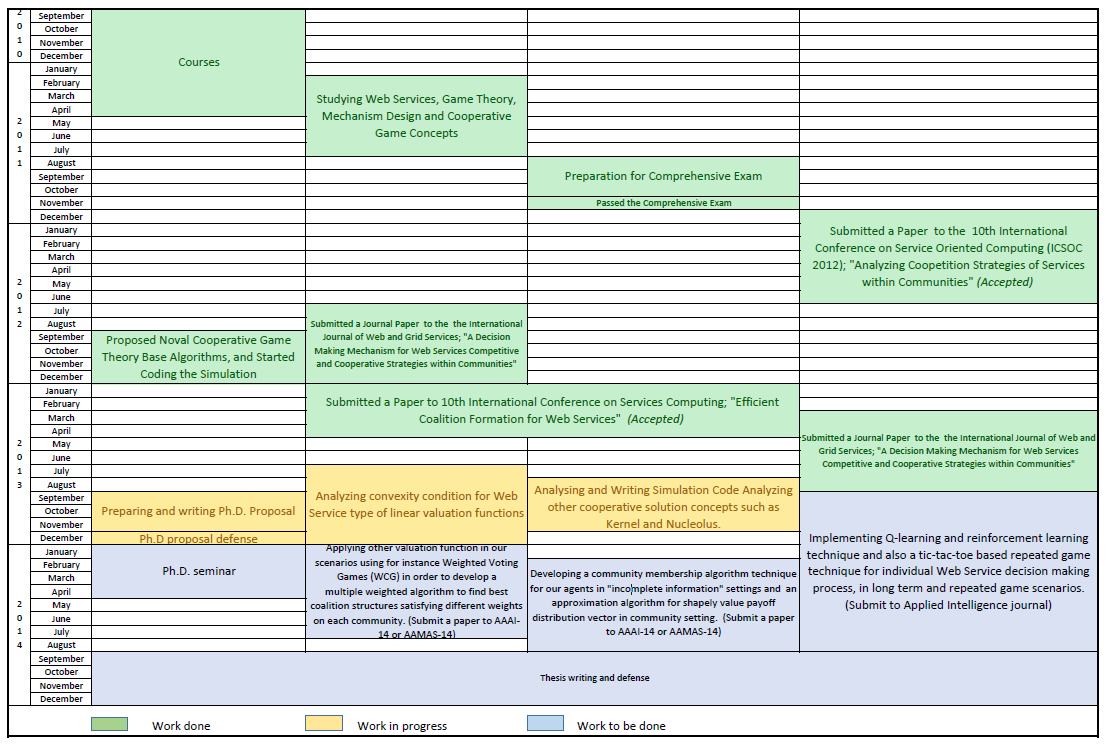
\includegraphics[width=1 \columnwidth]{figures/timetable.png}
%\includegraphics[width=16cm, height=21cm]{figures/figure6.eps}
%\caption{Schedule time of research} \label{figure6}
\end{center}
\end{figure}
    \end{frame}
%%%%%%%%%%%%%%%%%%%%%%%%%%%%%%%% frame27 Milestones %%%%%%%%%%%%%%%%%%%%%%%%%%%%%%%%%%%%%
%%%%%%%%%%%%%%%%%%%%%%%%%%%%%%%%%%%%%%%%%%%%%%%%%%%%%%%%%%%%%%%%%%%%%%%%%%%%%%%
%%%%%%%%%%%%%%%%%%%%%%%%%%%%%%%%%%%%
%%%%%%%%%%%%%%%%%%%%%%%%%%%%%%%%%%%%%%%%%%%%%%%%%%%%%%%%%%%%%%%%%%%%%%%%%%%%%%
\begin{frame}{Publications}

    \begin{enumerate}
        \item Published a paper in 10th International Conference on Services Computing; \emph{"Efficient Coalition Formation for Web Services"} {\color{blue} (Accepted)}
        \item Submitted a Journal Paper to the International Journal of Web and Grid Services; IEEE Transactions on Services Computing {\color{blue} (Second round of review)}
        \item Submitted a Paper to the 10th International Conference on Service Oriented Computing (ICSOC 2012); \emph{"Analyzing Coopetition Strategies of Services within Communities"} {\color{blue} (Accepted)}
        \item Submitted a Journal Paper to the International Journal of Web and Grid Services; IEEE Transactions on Services Computing; \emph{"To Compete or to Cooperate? This is the Question in Communities of Autonomous Services"}
    \end{enumerate}

%\centering
%\begin{itemize}
%\item \textbf{Questions Please !}
%\end{itemize}

\end{frame}

\end{document}
